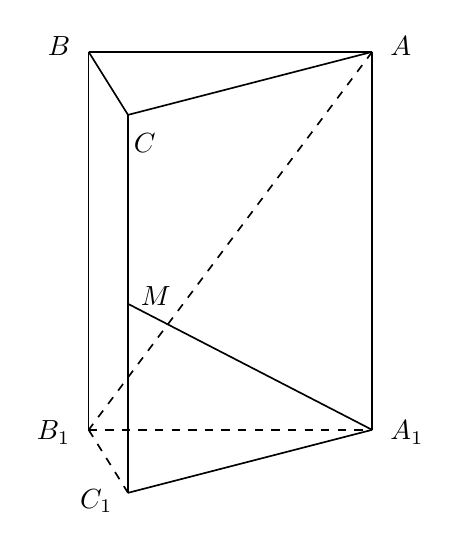
\begin{tikzpicture}[x=1cm,y=1cm,line width=.6pt]
% Right prism ABC-A1B1C1; M midpoint of CC1; diagonals AB1 (dashed), A1M (solid).
\coordinate (B) at (0,5.2);
\coordinate (A) at (3.6,5.2);
\coordinate (C) at (0.5,4.4);
\coordinate (Bone) at (0,0.4);
\coordinate (Aone) at (3.6,0.4);
\coordinate (Cone) at (0.5,-0.4);
\coordinate (M) at (0.5,2.0);
% top face
\draw (B) -- (A);
\draw (B) -- (C);
\draw (C) -- (A);
% bottom face
\draw[dashed] (Bone) -- (Aone);
\draw[dashed] (Bone) -- (Cone);
\draw (Cone) -- (Aone);
% laterals
\draw (B) -- (Bone);
\draw (A) -- (Aone);
\draw (C) -- (Cone);
% diagonals
\draw[dashed] (A) -- (Bone);
\draw (M) -- (Aone);
% labels offset clear of strokes
\node[left,xshift=-3pt,yshift=2pt] at (B) {$B$};
\node[right,xshift=3pt,yshift=2pt] at (A) {$A$};
\node[below,xshift=6pt,yshift=-3pt] at (C) {$C$};
\node[right=2pt,xshift=-1pt,yshift=3pt] at (M) {$M$};
\node[left,xshift=-3pt,yshift=-1pt] at (Bone) {$B_{1}$};
\node[left,xshift=-2pt,yshift=-3pt] at (Cone) {$C_{1}$};
\node[right,xshift=3pt,yshift=-1pt] at (Aone) {$A_{1}$};
\end{tikzpicture}
